%
% "The UCD CASL SenseTile System", for IEEE Pervasive Computing Joseph
% R. Kiniry, Vieri del Bianco, Dragan Stosic $Id: paper.tex 2795
% 2007-09-23 19:35:53Z dmz
%

\documentclass{article} \usepackage{times}

\usepackage{ifpdf} \usepackage{a4wide} \usepackage{pdfsync}

\ifpdf \usepackage[pdftex]{graphicx} \else \usepackage{graphicx} \fi

\usepackage{xspace} \usepackage{tabularx} \usepackage{epsfig}
\usepackage{amsmath} \usepackage{amsfonts} \usepackage{amssymb}
\usepackage{eucal} \usepackage{stmaryrd} \usepackage{float}
\usepackage{listings} % @(#)$Id: jml-listings.tex,v 1.6 2007/06/25 22:37:23 leavens Exp $
%
% Copyright (C) 2006 Iowa State University
%
% This file is part of JML
%
% JML is free software; you can redistribute it and/or modify
% it under the terms of the GNU General Public License as published by
% the Free Software Foundation; either version 2, or (at your option)
% any later version.
%
% JML is distributed in the hope that it will be useful,
% but WITHOUT ANY WARRANTY; without even the implied warranty of
% MERCHANTABILITY or FITNESS FOR A PARTICULAR PURPOSE.  See the
% GNU General Public License for more details.
%
% You should have received a copy of the GNU General Public License
% along with JML; see the file COPYING.  If not, write to
% the Free Software Foundation, 675 Mass Ave, Cambridge, MA 02139, USA.
%
% A JML listings environment.
%
% AUTHOR: Gary T. Leavens
%
% requires listings i.e., do \usepackage{listings} first
%
% This file is set up to be used via % @(#)$Id: jml-listings.tex,v 1.6 2007/06/25 22:37:23 leavens Exp $
%
% Copyright (C) 2006 Iowa State University
%
% This file is part of JML
%
% JML is free software; you can redistribute it and/or modify
% it under the terms of the GNU General Public License as published by
% the Free Software Foundation; either version 2, or (at your option)
% any later version.
%
% JML is distributed in the hope that it will be useful,
% but WITHOUT ANY WARRANTY; without even the implied warranty of
% MERCHANTABILITY or FITNESS FOR A PARTICULAR PURPOSE.  See the
% GNU General Public License for more details.
%
% You should have received a copy of the GNU General Public License
% along with JML; see the file COPYING.  If not, write to
% the Free Software Foundation, 675 Mass Ave, Cambridge, MA 02139, USA.
%
% A JML listings environment.
%
% AUTHOR: Gary T. Leavens
%
% requires listings i.e., do \usepackage{listings} first
%
% This file is set up to be used via % @(#)$Id: jml-listings.tex,v 1.6 2007/06/25 22:37:23 leavens Exp $
%
% Copyright (C) 2006 Iowa State University
%
% This file is part of JML
%
% JML is free software; you can redistribute it and/or modify
% it under the terms of the GNU General Public License as published by
% the Free Software Foundation; either version 2, or (at your option)
% any later version.
%
% JML is distributed in the hope that it will be useful,
% but WITHOUT ANY WARRANTY; without even the implied warranty of
% MERCHANTABILITY or FITNESS FOR A PARTICULAR PURPOSE.  See the
% GNU General Public License for more details.
%
% You should have received a copy of the GNU General Public License
% along with JML; see the file COPYING.  If not, write to
% the Free Software Foundation, 675 Mass Ave, Cambridge, MA 02139, USA.
%
% A JML listings environment.
%
% AUTHOR: Gary T. Leavens
%
% requires listings i.e., do \usepackage{listings} first
%
% This file is set up to be used via \input{jml-listings}.
% If you want, you could make a version that is a style file,
% but then change \lstdefinelanguage to \lst@definelanguage below.
%
\lstdefinelanguage[JML]{Java}[]{Java}%
       {% C++ style comments have to start with a blank!
        comment=[l]{//\ },
        % And C-style comments must also start with a blank or star!
        morecomment=[s]{/*\ }{*/},        
        morecomment=[s]{/**}{*/},
        % sensitive=true, % inherited
        % Add JML keywords as level 1 keywords, so can typeset differently
        classoffset=1,
        % And here are all the wonderful JML keywords
        morekeywords={abrupt_behavior,abrupt_behaviour,
         accessible,accessible_redundantly,also,assert,assert_redundantly,
         assignable,assignable_redundantly,assume,assume_redundantly,
         axiom,behavior,behaviour,breaks,breaks_redundantly,
         callable,callable_redundantly,captures,captures_redundantly,
         choose,choose_if,code,code_bigint_math,code_java_math,
         code_safe_math,constraint,constraint_redundantly,constructor,
         continues,continues_redundantly,decreases,decreases_redundantly,
         decreasing,decreasing_redundantly,diverges,diverges_redundantly,
         duration,duration_redundantly,ensures,ensures_redundantly,
         example,exceptional_behavior,exceptional_behaviour,
         exceptional_example,exsures,exsures_redundantly,extract,field,
         forall,for_example,ghost,helper,hence_by,hence_by_redundantly,
         implies_that,in,in_redundantly,initializer,initially,instance,
         invariant,invariant_redundantly,loop_invariant,
         loop_invariant_redundantly,maintaining,maintaining_redundantly,
         maps,maps_redundantly,measured_by,measured_by_redundantly,method,
         model,model_program,modifiable,modifiable_redundantly,modifies,
         modifies_redundantly,monitored,monitors_for,non_null,
         normal_behavior,normal_behaviour,normal_example,nowarn,
         nullable,nullable_by_default,old,or,post,post_redundantly,
         pre,pre_redundantly,pure,readable,refine,refines,refining,represents,
         represents_redundantly,requires,requires_redundantly,
         returns,returns_redundantly,set,signals,signals_only,
         signals_only_redundantly,signals_redundantly,spec_bigint_math,
         spec_java_math,spec_protected,spec_public,spec_safe_math,
         static_initializer,uninitialized,unreachable,weakly,
         when,when_redundantly,working_space,working_space_redundantly,
         writable
        },
        % keywords from the universe type system
        morekeywords={rep,peer,readonly},
        % typeset everything that starts with a backslash as a keyword
        % BUG: this doesn't allow typesetting these keywords differently
        keywordsprefix=\\,
        otherkeywords={<:,<-,->,..,<==,==>,<==>,<=!=>},
        classoffset=0 % restore default class for keywords
}
.
% If you want, you could make a version that is a style file,
% but then change \lstdefinelanguage to \lst@definelanguage below.
%
\lstdefinelanguage[JML]{Java}[]{Java}%
       {% C++ style comments have to start with a blank!
        comment=[l]{//\ },
        % And C-style comments must also start with a blank or star!
        morecomment=[s]{/*\ }{*/},        
        morecomment=[s]{/**}{*/},
        % sensitive=true, % inherited
        % Add JML keywords as level 1 keywords, so can typeset differently
        classoffset=1,
        % And here are all the wonderful JML keywords
        morekeywords={abrupt_behavior,abrupt_behaviour,
         accessible,accessible_redundantly,also,assert,assert_redundantly,
         assignable,assignable_redundantly,assume,assume_redundantly,
         axiom,behavior,behaviour,breaks,breaks_redundantly,
         callable,callable_redundantly,captures,captures_redundantly,
         choose,choose_if,code,code_bigint_math,code_java_math,
         code_safe_math,constraint,constraint_redundantly,constructor,
         continues,continues_redundantly,decreases,decreases_redundantly,
         decreasing,decreasing_redundantly,diverges,diverges_redundantly,
         duration,duration_redundantly,ensures,ensures_redundantly,
         example,exceptional_behavior,exceptional_behaviour,
         exceptional_example,exsures,exsures_redundantly,extract,field,
         forall,for_example,ghost,helper,hence_by,hence_by_redundantly,
         implies_that,in,in_redundantly,initializer,initially,instance,
         invariant,invariant_redundantly,loop_invariant,
         loop_invariant_redundantly,maintaining,maintaining_redundantly,
         maps,maps_redundantly,measured_by,measured_by_redundantly,method,
         model,model_program,modifiable,modifiable_redundantly,modifies,
         modifies_redundantly,monitored,monitors_for,non_null,
         normal_behavior,normal_behaviour,normal_example,nowarn,
         nullable,nullable_by_default,old,or,post,post_redundantly,
         pre,pre_redundantly,pure,readable,refine,refines,refining,represents,
         represents_redundantly,requires,requires_redundantly,
         returns,returns_redundantly,set,signals,signals_only,
         signals_only_redundantly,signals_redundantly,spec_bigint_math,
         spec_java_math,spec_protected,spec_public,spec_safe_math,
         static_initializer,uninitialized,unreachable,weakly,
         when,when_redundantly,working_space,working_space_redundantly,
         writable
        },
        % keywords from the universe type system
        morekeywords={rep,peer,readonly},
        % typeset everything that starts with a backslash as a keyword
        % BUG: this doesn't allow typesetting these keywords differently
        keywordsprefix=\\,
        otherkeywords={<:,<-,->,..,<==,==>,<==>,<=!=>},
        classoffset=0 % restore default class for keywords
}
.
% If you want, you could make a version that is a style file,
% but then change \lstdefinelanguage to \lst@definelanguage below.
%
\lstdefinelanguage[JML]{Java}[]{Java}%
       {% C++ style comments have to start with a blank!
        comment=[l]{//\ },
        % And C-style comments must also start with a blank or star!
        morecomment=[s]{/*\ }{*/},        
        morecomment=[s]{/**}{*/},
        % sensitive=true, % inherited
        % Add JML keywords as level 1 keywords, so can typeset differently
        classoffset=1,
        % And here are all the wonderful JML keywords
        morekeywords={abrupt_behavior,abrupt_behaviour,
         accessible,accessible_redundantly,also,assert,assert_redundantly,
         assignable,assignable_redundantly,assume,assume_redundantly,
         axiom,behavior,behaviour,breaks,breaks_redundantly,
         callable,callable_redundantly,captures,captures_redundantly,
         choose,choose_if,code,code_bigint_math,code_java_math,
         code_safe_math,constraint,constraint_redundantly,constructor,
         continues,continues_redundantly,decreases,decreases_redundantly,
         decreasing,decreasing_redundantly,diverges,diverges_redundantly,
         duration,duration_redundantly,ensures,ensures_redundantly,
         example,exceptional_behavior,exceptional_behaviour,
         exceptional_example,exsures,exsures_redundantly,extract,field,
         forall,for_example,ghost,helper,hence_by,hence_by_redundantly,
         implies_that,in,in_redundantly,initializer,initially,instance,
         invariant,invariant_redundantly,loop_invariant,
         loop_invariant_redundantly,maintaining,maintaining_redundantly,
         maps,maps_redundantly,measured_by,measured_by_redundantly,method,
         model,model_program,modifiable,modifiable_redundantly,modifies,
         modifies_redundantly,monitored,monitors_for,non_null,
         normal_behavior,normal_behaviour,normal_example,nowarn,
         nullable,nullable_by_default,old,or,post,post_redundantly,
         pre,pre_redundantly,pure,readable,refine,refines,refining,represents,
         represents_redundantly,requires,requires_redundantly,
         returns,returns_redundantly,set,signals,signals_only,
         signals_only_redundantly,signals_redundantly,spec_bigint_math,
         spec_java_math,spec_protected,spec_public,spec_safe_math,
         static_initializer,uninitialized,unreachable,weakly,
         when,when_redundantly,working_space,working_space_redundantly,
         writable
        },
        % keywords from the universe type system
        morekeywords={rep,peer,readonly},
        % typeset everything that starts with a backslash as a keyword
        % BUG: this doesn't allow typesetting these keywords differently
        keywordsprefix=\\,
        otherkeywords={<:,<-,->,..,<==,==>,<==>,<=!=>},
        classoffset=0 % restore default class for keywords
}

\lstset{language=[JML]Java,xleftmargin=20pt,xrightmargin=20pt}

\ifpdf \usepackage{epstopdf}
\usepackage[pdftex,bookmarks=false,a4paper=false,
plainpages=false,naturalnames=true, colorlinks=true,pdfstartview=FitV,
linkcolor=blue,citecolor=blue,urlcolor=blue, pdfauthor="Joseph
R. Kiniry and Vieri del Bianco"]{hyperref} \else
\usepackage[dvips,linkcolor=blue,citecolor=blue,urlcolor=blue]{hyperref}
\fi

\newcommand{\tablesize}{\footnotesize} \newcommand{\eg}{e.g.,\xspace}
\newcommand{\ie}{i.e.,\xspace} \newcommand{\etc}{etc.\xspace}
\newcommand{\myhref}[2]{\ifpdf\href{#1}{#2}\else\htmladdnormallinkfoot{#2}{#1}\fi}
\newcommand{\myhreffootnote}[3]{\myhref{#1}{#2}\footnote{#3
    \myhref{#1}{#1}}}

\newcommand{\lil}[1]{\texttt{\lstinline|#1|}}

% \newcommand{\notev}[1]{\xspace$\textcolor{blue}{\omega^\textsf{vieri}}$\marginpar{\scriptsize\textsf{Vieri:}
%     #1}}
\newcommand{\notev}[1]{\xspace\marginpar{\scriptsize\textsf{Vieri:}
    #1}}
\newcommand{\notej}[1]{\xspace$\frac{\varocircle}{\textsf{jk}}$\marginpar{\scriptsize\textsf{Joe:}
    #1}}
\newcommand{\noted}[1]{\xspace$\textcolor{red}{\dagger^\textsf{dragan}}$\marginpar{\scriptsize\textsf{Dragan:}
    #1}}

\newcommand{\todo}[1]{\texttt{\textbf{TODO:} #1}}

\newcommand{\ST}{\emph{SenseTile}\xspace}
\newcommand{\SB}{\emph{Sensor Board}\xspace} \newcommand{\STSB}{\ST
  \SB\xspace} \newcommand{\STSBs}{\ST \emph{Sensor Boards}\xspace}
\newcommand{\STPU}{\ST \emph{Processor Unit}\xspace}
\newcommand{\STPUs}{\ST \emph{Processor Units}\xspace}
\newcommand{\STU}{\ST \emph{Unit}\xspace} \newcommand{\STUs}{\ST
  \emph{Unit}\xspace}

\newcommand{\STs}{\emph{SenseTiles}\xspace}

\newcommand{\simulator}{\STSB \emph{Simulator}\xspace}

\newcommand{\datastore}{\ST Scientific Datastore\xspace}
\newcommand{\computefarm}{The \ST Scientific Compute Farm\xspace}
\newcommand{\computefarmlong}{UCD CASL \ST Software and Data Compute
  Server Farm\xspace} \newcommand{\sensorfarm}{The \STSBs\xspace}

% ---------------------------------------------------------------------
% New commands, macros, \etc
% ---------------------------------------------------------------------

%% \input{kt}

% =====================================================================

\begin{document}

\title{Deriving an Executable Model of a Data Stream Protocol from its
  Specification}

\maketitle

% ======================================================================
% \thispagestyle{empty}

% ======================================================================
\section{Introduction}
\label{sec:introduction}

The \textbf{UCD CASL SenseTile System} is a large-scale,
general-purpose sensor system to be installed at the University
College Dublin in Dublin, Ireland.  Our facility aims to provide a
scalable and extensible infrastructure for performing in-depth
investigation of both the specific and general issues in large-scale
sensor networking.

Because of hard time constraints, and the initial unavailability of
the custom board, we needed to progress concurrently with all the
development tasks:

\begin{itemize}
\item specification of the communication protocol;
\item development of the physical board specification and following
  realization;
\item development of the board embedded software;
\item development of the software driver to communicate with the
  board;
\item development of the software simulators of the board.
\end{itemize}

The development of the physical board, along with its embedded
software, has been done by an external manufacturer, thus it is not
directly taken into account here.

There exist various approaches in literature addressing this kind of
development constraints (rapid development in hardware software
co-design), but they are all focused on big-scale systems
\cite{Slomka2000,Hoffman2001}.

Even when considering the development of the device hardware, embedded
software and software driver as separate entities, that possibly have
to be developed concurrently, the approaches proposed are similar in
structure to the one seen in the case of hardware software
co-design\cite{Valderrama1995,Siegmund2002,Ryzhyk2009}: they all focus
on a specification that aims to be as complete as possible.

This approach has been considered not feasible nor convenient if
applied to our case since it does not respect some of the
requirements: first of all, we want to develop all the software
components concurrently, we want to enhance the protocol specification
incrementally and we are not able to provide a complete specification
from the beginning, hence, a properly defined specification is not
available in advance. Secondly, we are not interested in direct code
generation from specification, since we do not want to have any
dependencies on code generators; in fact the programming language to
be used to develop the driver has been postponed for a while.

To tackle the complexity of the concurrent development tasks, the
formal model of the protocol was used as a focus point that led all
the other development tasks. As it can be seen, the central role of
the specification is unchanged; what is changed is how and when the
specification is developed.

The protocol to specify has been divided in various (thin) layers,
each of the layer has been specified with a different lightweight
approach: some of the layers have been specified formally, while
others have been specified in an unprecise way.  The formal
specifications have been used to check at run time the correctness of
the \SB, the driver and the simulators.  The formal specifications
have also been used to automatically generate a test suite to verify
the driver and the simulators, and eventually to verify the
specification itself.  An hand made test suite has been used to verify
the driver and the simulators as well.  The generated and hand made
test suites have been used together, complementing each other.

The approach proved itself effective, at the point that, when the
board has been finally released, only one small defect has been found
in the driver, while the errors and not agreed changes introduced in
the board and in the protocol it implemented, have been discovered
immediately, with no additional effort.  Besides, the simulators are
able to feed with correct data the rest of the system.


% =====================================================================
\section{Data stream and protocol description}
\label{sec:data_stream_and_protocol_description}

A custom protocol has been developed to manage the entire \STSB, built
on top of a USB serial channel; the protocol main function is to read
sensor data and control the \SB.  The protocol is asynchronous and
packet based, the packets have a fixed length.  The protocol has been
divided in multiple layers to ease its formal description.

We will examine the output sensor data packet.  The packet byte and
info structures of the output sensor data packet reflect the board
capabilities and built in sensors.  Essentially a single packet has to
accommodate various types of data streams chunks.



% =====================================================================
\section{Data stream and protocol specification}
\label{sec:data_stream_and_protocol_specification}

The specifications of the protocol has been used as a central point to
lead all the other development tasks.

Regarding the formal specification used, we needed a specification
capable of:

\begin{itemize}
\item Be executed at run time: if something on the protocol is not
  respected, the run time execution environment is capable to detect
  and signal the fault.
\item Generate tests.
\item Verify simulators.
\item Be used in conjunction of hand written unit tests.
\end{itemize}

\paragraph{Packet byte structure specification}

The specification is provided by a hand made test suite, composed of
unit and integration tests; the tests specifies the behaviors of the
Java implementation, which is capable of recognizing the proper packet
structure in a binary data stream. The implementation is tricky: it
checks for the sentinels repeatedly to be sufficiently confidant that
the byte stream can be properly decomposed into a packet stream.

Fulfilled requirements:

\begin{itemize}
\item The specification cannot be checked at run time.
\item Meaningful automatic tests cannot be generated.
\item The specification can be used to verify a packet byte structure
  simulator.
\item The implementation were actually driven (Test Driven
  Development) by the test suite specification.
\end{itemize}

\paragraph{Packet info structure specification}

The specification is provided by JML annotations\cite{JML2}\footnote{
  \myhref{http://www.cs.ucf.edu/~leavens/JML/}{The Java Modeling
    Language (JML)}} and by a hand made test suite.

Many tools are able to support JML specification language are
available, focusing on different aspects of the language.  JML2 suite
of tools\cite{BurdyEtal05-STTT}
\footnote{\myhref{http://sourceforge.net/projects/jmlspecs/}{Common
    JML tools}} has been chosen, since the suite provides both run
time verification support and test generation support.

Fulfilled requirements:

\begin{itemize}
\item The Java API specification part is checked automatically by the
  Java compiler, while the JML specification part can be checked at
  run time using the provided JML2 run time environment.
\item Meaningful automatic tests can be generated from the JML
  specification.
\item The JML specification can be used to verify a simulator, which
  generates packets as the real board would do .The specification can
  also be used to verify the real driver implementation, based on the
  packet byte structure implementation presented above.
\item The implementation was driven by the formal JML specification
  and by the hand made test suite.  Finally, hand made unit tests can
  be checked, during execution, against the formal specification,
  using the provided JML2 run time environment.
\end{itemize}

\paragraph{Single packet rules}

The specification is provided exclusively by the formal specification
with JML language.

The fulfilled requirements of a JML specification have been already
described in the previous paragraph, that is:

\begin{itemize}
\item The JML specification is checkable at run time.
\item Tests can be automatically generated.
\item Simulators can be verified.
\item The specification can be used with hand written tests.
\end{itemize}

\subsection{On simulators}
\label{subsec:on_simulators}

Simulators can be used to test parts of the system, to minimizing
their dependencies: a simulator can be used by upper layers, with no
need to provide the functionalities of the lower layers.  During the
development of the \STSB the simulators have been essential, since the
physical board was not available: we needed at least to remove the
dependencies over the real board to execute the driver implementation.
Simulators have been built concurrently with the specification, the
driver implementation, and the tests.

Theoretically a separate simulator should be needed for each protocol
layer: this would enable us to specify, develop and test each layer in
isolation.  In our case we evaluated not worth the effort to replicate
the layer structure into simulators; the choice was motivated by the
fact that such a distinction would have not provided us any
perceivable benefit.  Two simulators were built.

The simulators have been built reflecting the software abstraction
layers defined for the driver.  The driver API is splitted in two
abstraction layers: the general high level interfaces, that expose the
main functionalities of the board and the main contents of the
packets, and the lower level implementation that parse the data
streams in and out the board, meant to translate the higher level
instructions and data in properly formed packets.

The high level simulator implements the interfaces providing the
methods to deal with an abstracted \SB: the simulator knows nothing
about the details of the real format of the binary data streams.  The
low level simulator is capable to rebuild the \SB data streams: the in
and out data streams are built exactly as the sensor board is expected
to be able to parse or generate.

\subsection{JML specification examples}
\label{subsec:a_jml_specification_example}

The JML specifications that have been written are of varying
complexities.  Some of the specifications are simple, focusing on
constraints that should hold when calling a method (the preconditions)
and constraints on the return value (the very basic form of
postconditions).  In listing \ref{lst:jml_example_simple} a simple JML
specification example is shown, the method \lil{getTemperature} is
declared to be \lil{/*@ pure @*/}, which means that it cannot change
the state of any object (a postcondition), the specification also
constraints the return value with a lower and upper bound (another
postcondition).

\begin{lstlisting}[
  caption={A simple specification with JML annotation: simple postconditions.},
  label=lst:jml_example_simple,
  float=htbp]
  /*@ ensures \result >= -880; ensures \result <= 2047; @*/ /*@ pure
  @*/ short getTemperature();
\end{lstlisting}

\sloppy

Some of the specifications are rather complex, usually focusing on
properties regarding the behavior of a whole object.  In listing
\ref{lst:jml_example_invariant} a complex invariant example is shown;
an invariant is a property that has to be maintained during the life
cycle of an object, more precisly, an invariant is assumed on entry
and guaranteed on exit of each method of an object.  The invariant is
constraining the number of samples for each medium data rate streams:
the total number of streams is \lil{Frame.ADC_CHANNELS}, the total
number of frames is \lil{FRAMES}, the constant constraining the number
of samples is \lil{FRAMES/Frame.ADC_CHANNELS+1}, meaning that the
samples contained in a frame are fairly distributed on the channels.
The valid samples are counted parsing all the frames contained in a
packet, selecting only the matching valid samples.  A medium data rate
stream sample is considered valid when \lil{isADCActive()} method
returns \lil{true}.

\fussy

\begin{lstlisting}[
  caption={A specification with JML annotation: a complex object invariant which constraints 
    the number of samples for each medium data rate stream channel.},
  label=lst:jml_example_invariant,
  float=htbp]
  /*@ invariant ( \forall int channel; 0 <= channel && channel <
  Frame.ADC_CHANNELS; ( \num_of int i; 0<= i && i<(FRAMES-1); (
  getFrame(i).isADCActive() && (getFrame(i).getADCChannel() ==
  channel) ) ) <= (FRAMES / Frame.ADC_CHANNELS + 1) ); @*/
\end{lstlisting}



% =====================================================================
\section{Test cases}
\label{sec:test_cases}

The unit test cases that have been built to verify the protocol driver
are of two kinds: hand made unit tests and automatically generated
unit tests based on JML specifications.  The tests have been thought
to be used together, they are complementary.  The tests effectiveness
has been evaluated for each test suite; the evaluation is carried out
in section \ref{sec:test_cases_retrospectives}.  The test
effectiveness evaluation has been based on three elements: effective
results on piloting the real board (quantitative), code coverage
(quantitative), development help and usefulness (qualitative).

Hand made unit tests specifies the behavior not specified by formal
specification; nevertheless this is not the only purpose they have.
Hand made unit tests have been used to drive the development, since
the Test Driven Development approach\cite{beck2003test} has been
followed during development.

\paragraph*{Hand made tests}

The package structure of the driver developed is shown in Figure
\ref{fig:class_diagram_main}: two independent packages has been
defined (\lil{Stream} and \lil{Driver}).  The packages are abstract,
that is, they mainly contain abstractions; in Java language this is
translated into a package which contains mainly abstract classes or
interfaces.  The two abstract packages have various implementations,
and the dependency between the two is not direct, since it is realized
through an implementation (\lil{StreamDriver}).  This is needed to
maintain a high decoupling of the packages, and is the result of
applying the classical dependency inversion
principle\cite{martin1996dependency}: the dependency structure of the
packages has a saw shape, a common shape on systems where the
dependency inversion principle has been followed.

\begin{figure}[htb!]
  \centering
  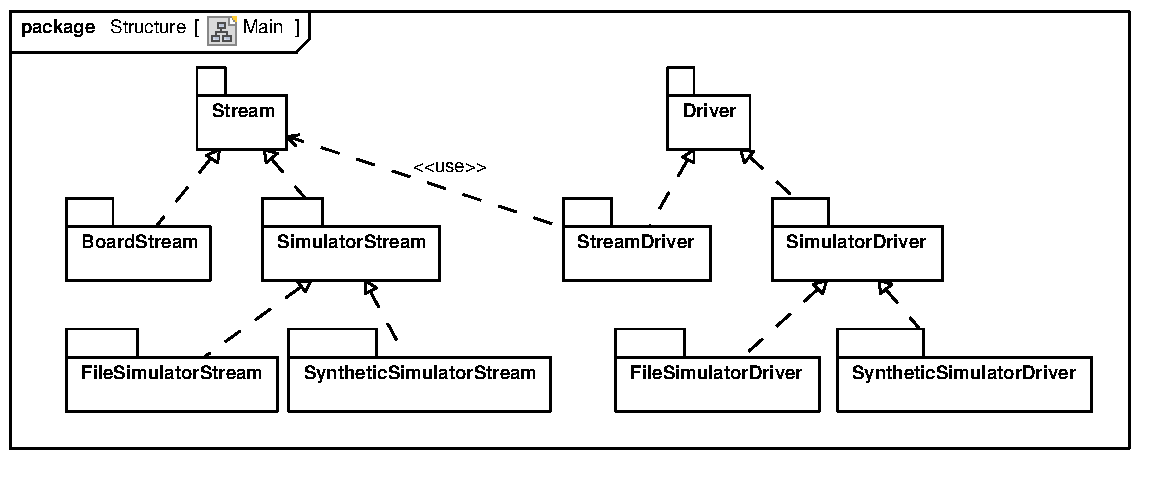
\includegraphics[scale=0.7]{UML_model/Class_Diagram__Structure__Main}
  \label{fig:class_diagram_main}
  \caption{Main packages class diagram.}
\end{figure}

The test package structure, which is shown in Figure
\ref{fig:class_diagram_test} reflects and mimics the code structure;
the tests for an abstract package are abstract, to be implemented by
the package that tests a corresponding system implementation; this is
a well known test pattern (the Abstract Test
Pattern\cite{thomas2004java}) used to test that the contracts are
respected in the implementations.  For instance, package \lil{DriverT}
contains abstract tests for the abstractions of package \lil{Driver},
package \lil{StreamDriverT} inherits the abstractions contained in
\lil{DriverT} and makes them concrete, to test the corresponding
implementation \lil{StreamDriver}; package \lil{StreamDriverT} also
contains stand alone tests written specifically for the implementation
contained in \lil{StreamDriver}.

\begin{figure}[htb!]
  \centering
  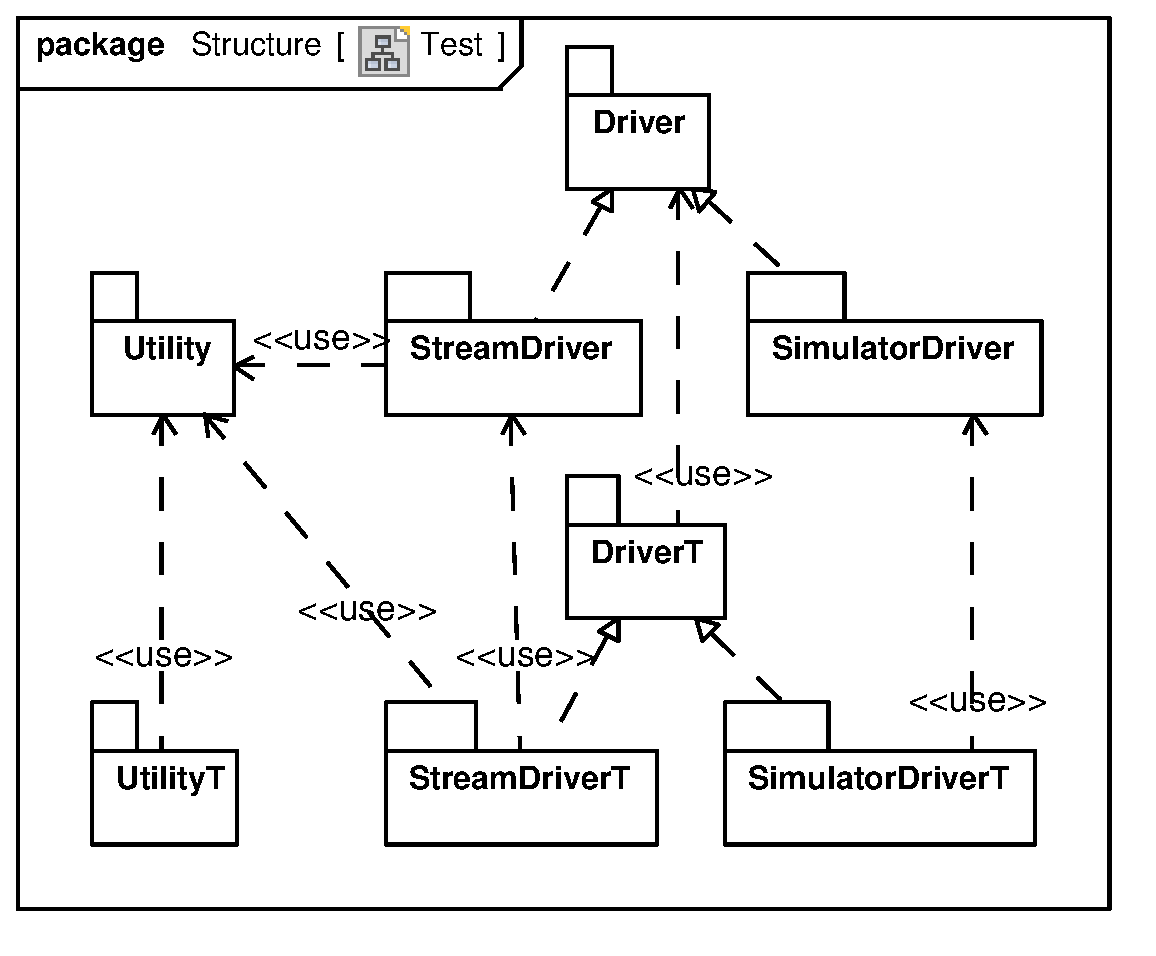
\includegraphics[scale=0.4]{UML_model/Class_Diagram__Structure__Test}
  \label{fig:class_diagram_test}
  \caption{Test packages class diagram.}
\end{figure}

\paragraph*{Generated tests}

The JML specification has been used to generate the tests.  A specific
tool of the JML2 suite is able to automatically generate
them\cite{Cheon-Leavens02}.

The resulting test package structure is shown in Figure
\ref{fig:class_diagram_generatedtest}.  The package dependencies are
defined by the specifications; for instance, \lil{SimulatorDriverST}
are generated tests, they test (hence use) the implementation
\lil{SimulatorDriver}, and have been generated using the corresponding
specification \lil{SimulatorDriverS}.  The generated tests do not
maintain the inheritance structure of the code and the specification.

\begin{figure}[htb!]
  \centering
  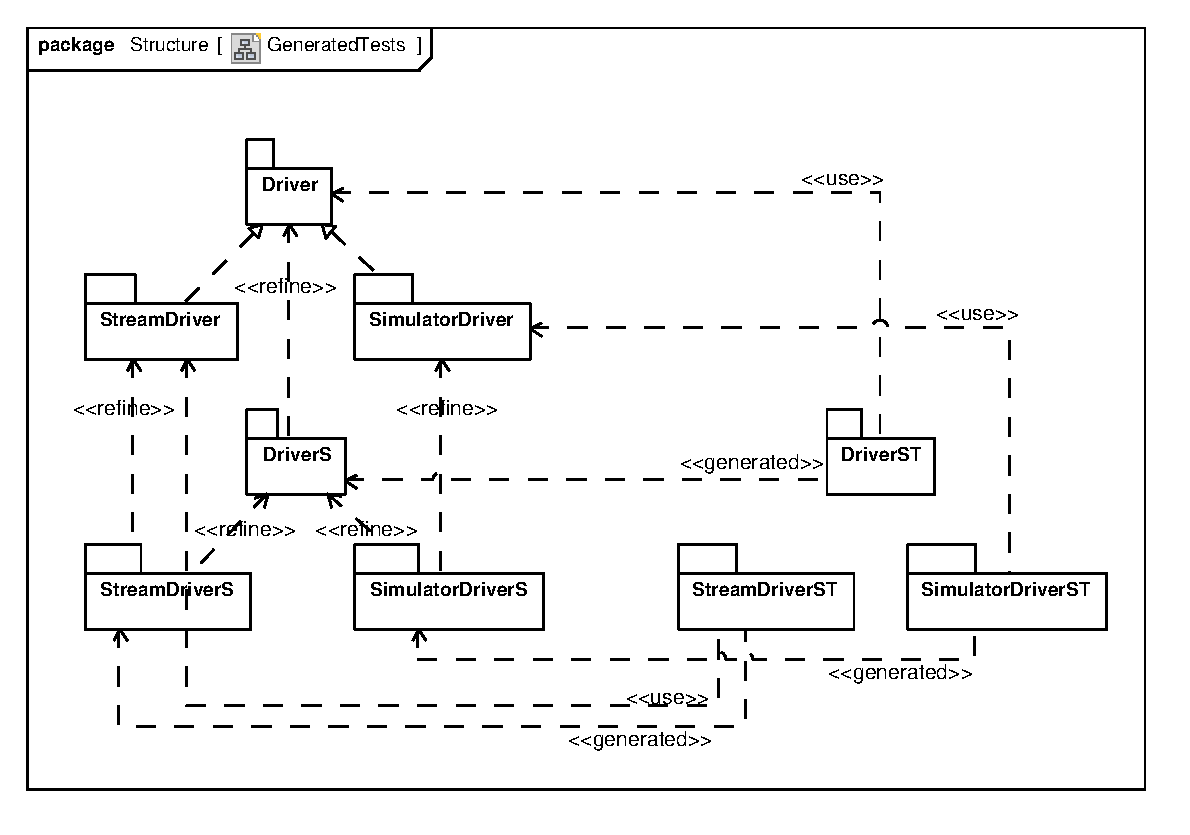
\includegraphics[scale=0.7]{UML_model/Class_Diagram__Structure__GeneratedTests}
  \label{fig:class_diagram_generatedtest}
  \caption{Generated test packages class diagram.}
\end{figure}

\paragraph*{On simulators, again}

A proper stub, driver and oracle should be identified for each method
under test to have proper unit test suite; stub, driver and oracle are
the usual components found in the harness that enable test
execution\cite{Binder1999}.  In
JUnit\footnote{\myhref{http://www.junit.org/}{JUnit}}, which is the
framework used to manage the implementation and execution of hand made
and generated unit tests, there is no clear distinction between
drivers, stubs, and oracles; none-less, even if a proper distinction
is not imposed by the framework, the conceptual distinction still
holds.

Hence, to properly unit test a package, we need:

\begin{description}
\item[Stub or Skeleton]: a piece of code that simulates the activity
  of the modules that are not under tests.
\item[Driver]: a piece of code that calls in a proper way the module
  under test.
\item[Oracle]: a mechanism used for determining whether a test has
  passed or failed, comparing the output of the module under test to
  the output the oracle determines the module should have.
\end{description}

Hand made unit tests and JML generated tests differ in how these
components are provided.  The distinctions and similarities are
summarized in Table \ref{tab:test_harness}.

\begin{table}[htbp]
  \caption{Hand made and generated tests harness.}
  \label{tab:test_harness}
  \begin{center}
    \begin{tabular}{|l|l|l|}\hline
      & \textbf{\textit{hand made}} & \textbf{\textit{JML}} \\\hline
      \textbf{\textit{Stub}} & to be provided & to be provided\\\hline
      \textbf{\textit{Driver}} & to be provided & automatic: 1 call\\\hline
      \textbf{\textit{Oracle}} & to be provided & 
      automatic: runtime assertion checker\\\hline
    \end{tabular}
  \end{center}
\end{table}

A module simulator can be used to ease the tasks of developing each
component of a test harness: it can be used as a stub, to simulate a
module needed by the module under test, it can be used as a driver, to
stimulate the module under test, it can be used as an oracle, if it
simulates the module under test.

In our system, the simulators has been used as stubs, so that we have,
during testing, a structure like the one shown in Figure
\ref{fig:class_diagram_streamdriver_test}.  In Figure
\ref{fig:class_diagram_streamdriver_test} the test suite
\lil{StreamDriverT} is using the \lil{SimulatorStream} to properly
simulate the \lil{Stream} used by \lil{StreamDriver}, which is the
system under test.

\begin{figure}[htb!]
  \centering
  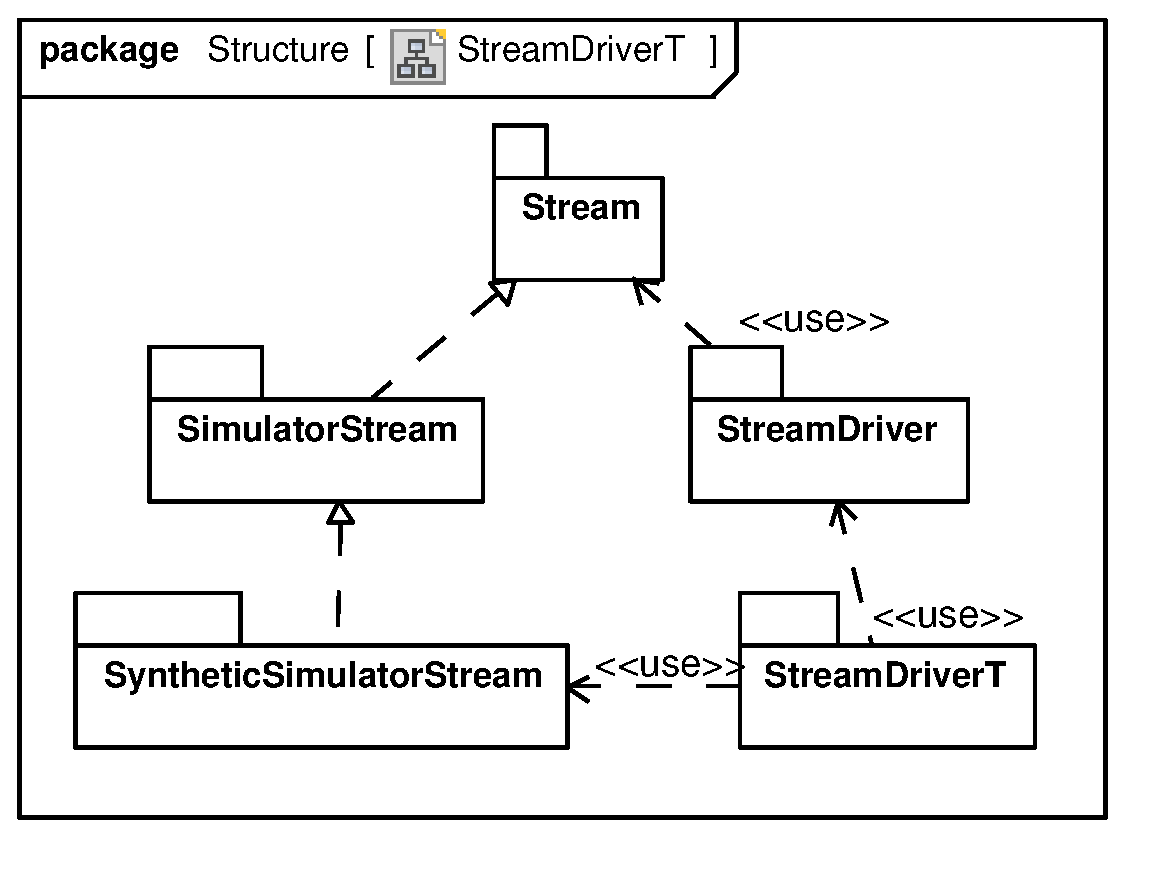
\includegraphics[scale=0.4]{UML_model/Class_Diagram__Structure__StreamDriverT}
  \label{fig:class_diagram_streamdriver_test}
  \caption{StreamDriver test packages class diagram: use of the stream
    simulator.}
\end{figure}

In our case, the use of simulators to enable unit testing, has been
essential to test the \STSB driver, since the physical board was not
available.  The simulators were have been used in both the hand made
and the generated test suite, since both of them need a proper set of
stubs to be executed.



% =====================================================================
\section{Test cases on the job}
\label{sec:test_cases_on_the_job}

The first prototype delivered was meant to build packets with values
taken from real sensors installed on the board.  The only sensors that
were not yet working were the sensors devoted to the fast rate data
streams, the audio sensors.  Only one error needed to be corrected in
the driver implementation, because of a (rare) combinations of
conditions that were not covered by the test cases, but that
occasionally showed up during real use.  One error have been
discovered in the low level system driver that the developed driver
was using (the system driver was outside of our development scope); to
eliminate the error an upgrade of the low level driver to a new
unreleased version was necessary.  No other errors were detected on
the driver side.

The prototype respected the packet byte structure
specification, but was not fully compliant to the packet info
structure specification and the single packet rules.  The formal model
and the run time assertion checker enabled the detection of these
errors.  4 protocol errors regarding the packet info structure
specification, and 2 protocol errors regarding the single packet rules
has been found. No other errors, except the mentioned ones, have been
later on discovered.

The hand made test suite is composed by over 140 tests, while the
generated one is 100 times bigger, totaling over 14000 tests.

We analyzed the test suites with
statement code coverage \footnote{The tool
  used to obtain statement code coverage metrics is
  \myhref{http://emma.sourceforge.net/}{Emma}.}: statement coverage
reports whether each executable statement has been encountered. 
The coverage results are reported
in the Table \ref{tab:statement_code_coverage}.

\begin{table}[htbp]
  \caption{Statement code coverage result, categorized by source package.}
  \label{tab:statement_code_coverage}
  \begin{center}
    \begin{tabular}{|c|c|c|c|}\hline
      & \textbf{\textit{hand}} & \textbf{\textit{generated}} &
      \textbf{\textit{total}} \\\hline
      \textbf{\textit{Driver}} & $15.9 \%$ & $6.3 \%$ & $15.9 \%$ \\\hline
      \textbf{\textit{StreamDriver}} & $76 \%$ & $79.7 \%$ & $88.5 \%$ \\\hline
      \textbf{\textit{SimulatorDriver}} & $64.9 \%$ & $44.2 \%$ &
      $71.2 \%$ \\\hline
      \textbf{\textit{Utility}} & $98.1 \%$ & $74.5 \%$ & $98.1 \%$ \\\hline
    \end{tabular}
  \end{center}
\end{table}



% =====================================================================
\section{Retrospective on test cases effectiveness}
\label{sec:test_cases_retrospectives}

The coverage measures reported in Table
\ref{tab:statement_code_coverage} are not high, in absolute
values. This is because of two different effects: non public methods,
and interfaces. 

But the combination of test suites is interesting, indicating that one
test suite is not completely overlapping the other: the test suites
are not to be considered alternatives, but they have to be used
together to achieve the higher benefits, they are complementary.

The test suites gave their best when used in a combined approach: the
generated test suite, checking simpler behaviors, and the hand made,
checking the more complex ones.


% ======================================================================
%% \nocite{ex1,ex2}
\bibliographystyle{latex8} \bibliography{extra,%
  abbrev,%
  ads,%
  category,%
  complexity,%
  hypertext,%
  icsr,%
  knowledge,%
  languages,%
  linguistics,%
  meta,%
  metrics,%
  misc,%
  modeling,%
  modeltheory,%
  reuse,%
  rewriting,%
  softeng,%
  specification,%
  ssr,%
  technology,%
  theory,%
  web,%
  upcoming,%
  upcoming_conferences,%
  conferences,%
  workshops,%
  verification,%
  escjava,%
  jml,%
  nijmegen}

% ======================================================================
% Fin

\end{document}



%%% Local Variables: 
%%% mode: latex
%%% eval: 
%%% TeX-master: t
%%% End: 
